% NCSU, CSC 522, Fall 2018
% Dr. Min Chi
% Project, Group 6

\documentclass{article}

\usepackage[final]{nips_2018}

\usepackage{natbib}

\usepackage[utf8x]{inputenc} % allow utf-8 input
\usepackage[T1]{fontenc}    % use 8-bit T1 fonts
\usepackage{hyperref}       % hyperlinks
\usepackage{url}            % simple URL typesetting
\usepackage{booktabs}       % professional-quality tables
\usepackage{amsfonts}       % blackboard math symbols
\usepackage{nicefrac}       % compact symbols for 1/2, etc.
\usepackage{microtype}      % microtypography
\usepackage{graphicx}
\usepackage{courier}
\usepackage{amsmath}
\usepackage{float}
\usepackage{subfig}
\usepackage{hyperref}

\title{Using Machine Learning to Predict NBA Outcomes}

\author{
Christopher Bailey \\
%Statistics \\
%NCSU \\
%Cary, NC \\
\texttt{{\tiny cdbaile7@ncsu.edu}} \\
\And 
Eleanor Schlechter \\
%Data Science \\
%NCSU \\
%Cary, NC\\
\texttt{{\tiny esschlec@ncsu.edu}} \\
\And 
Sakthi Murugan \\
%Computer Science \\
%NCSU \\
%Raleigh, NC \\
\texttt{{\tiny srmuruga@ncsu.edu}} \\
\And 
Shaohan Wang \\
%Mechanical Engineering \\
%NCSU \\
%Raleigh,  NC\\
\texttt{{\tiny swang62@ncsu.edu}} \\
}

\begin{document}

\maketitle

\begin{abstract}
  Future NBA outcomes can be accurately predicted with modern machine learning techniques. 
  This paper concentrates on the classification and regression techniques taught in the Automated Learning and Data Analysis graduate course at North Carolina State University; in particular Decision Trees, Naive Bayes, Artificial Neural Networks, and Support Vector Machine will be used to predict a dichotomous response of a player making the playoffs independent of the other members of the team or the team's overall performance, while Support Vector Regression and Linear Regression will be used to predict a continuous response of an individual player's salary based on their performance measures and qualities. 
\end{abstract}

\section{Background}
Quantitative analysis of sports has always been an attractive subset in statistics among the sports enthusiastic statisticians. 
Experts have focused on turning historical records of game statistics into useful information for decades. 
In the early days, forecasting game outcomes applied simple principles of statistics by combining some technical features of the games; however, the accuracy of these predictions had limitations. 
With advancements of machine learning techniques and the development of systems that aid scientific data sharing, researchers such as Fusheng Wang and Cristobal Vergara-Niedermayr \cite{Wang}, have leveraged these improvements to increase the accuracy in these predictions. 
Powerful data mining tools have enabled owners, managers, coaches and analysts alike, to find some interesting insights, which have not yet been explored. 
The games sponsored by the National Basketball Association (NBA) have been at the forefront of such research. 
An example of this research would be the Advanced Scout \cite{Bhandari} data mining application to predict the success of NBA teams. 
Another example is Bernard, Earl, and Kenneth's \cite{Bernard} work, in which the team has used varying types of neural networks to predict the success of NBA teams, concluding with an accuracy of over 70\%. 
Miljkovic, Gajic, and Kovacevic \cite{Miljkovic} have applied the Naive Bayes method to predict the outcome of a two team match-up by calculating the spread of each game by using a flavor of linear regression.

As it can be observed above, the main goal of sports analytics is to predict the overall, potential success of each team throughout each season. 
The obvious reason to support the investment in this space is the application of this data towards the team's preparation for an upcoming game. 
This data can pinpoint a team's weaknesses and show how they can be exploited in a match-up, or furthermore, which players in specific attribute most to said weaknesses. 
With that said, it became clear through ample research that each individual player's statistics have not been given focus in much of the NBA related machine learning studies. 
Following this train of thought, this paper will concentrate on the players's statistics to develop thoughtful predictions as to a team's performance as well as the efficiency of each player. 

Decision Trees, Naive Bayes, Artificial Neural Networks, and Support Vector Machine will be used to predict a dichotomous response of a player making the playoffs independent of the other members of the team or the team's overall performance, while Support Vector Regression and Linear Regression will be used to predict a continuous response of an individual player's salary.

\section{Proposed Methods}

In this experiment, both parametric and non-parametric predictions for both classification and regression were used.
Features have been selected to predict if a player will make it to the playoffs as well as their remuneration.

\subsection{Classification} 
Classification is a type of supervised learning in which the need is to label the data or assign each object to a category. In relation to predicting NBA outcomes, classification algorithms, such as Decision Trees, Naive Bayes, Artificial Neural Networks, and Support Vector Machine, will be predicting whether or not a player will make it into the playoffs.

\textbf{\textit{Decision Trees}} are incredibly intuitive and give much insight into which features in the data set are most important to the class label based on their location in the tree, which in this case will be top-down. 
Since this model is being applied to NBA data, which is composed of a number of continuous values, these chosen features were discretized prior to building the model. 
Once the data was prepared, the building of the tree began by using the Gini Index to decide where each node should be placed. 
Since over-fitting a decision tree is a large disadvantage of this approach, post-pruning will be performed and checked with cross validation to decide if a node should be "pruned" and changed to a leaf node. 

\textbf{\textit{Artificial Neural Networks}} were developed in the 1950s as an attempt to simulate the network of neurons that make up a human brain. 
With that said, the idea is for a computer to have the ability to learn things and make decisions in a "human-like" manner. 
This model will take features from the data set for each player as input, while in the the background, the model will constantly be changing the weight of each node to verify the result using the training data. 
After the training process is complete, the model will then consume the testing data to testify if the model will successfully predict if a player will make the playoffs within a relative good enough accuracy.


\textbf{\textit{Support Vector Machine}} is a supervised learning model for both classification and regression. 
The training algorithm builds a model that assigns new
examples to one category or the other, making it a nonprobabilistic binary linear classifier.
Kernels and soft margins can be used to classify data that are not linearly separable.
Support Vector Machines, unlike NN, do not start with random numbers, instead having a simple mathematical basic: find the maximal margin classifier. This is a straightforward quadratic programming problem, and can be plugged into any QP solver. 
There are two issue, one is that the data will not be linearly separable, the other that the QP time is big-Oh of $n^3$, reducing to a few iterations solving a linear system. To address the former we used radial basis function kernels, but are then faced with the tasks of choosing the optimal variance term, i.e. for 
$$
K(x,x') = \exp \left( - \frac{||x-x'||^2}{2\sigma^2} \right)
$$

what is the optimal value of $\sigma$. As shown in the classroom presentation, given ground truth and data
\begin{figure}[H]
    \centering
    \subfloat[Ground truth]{{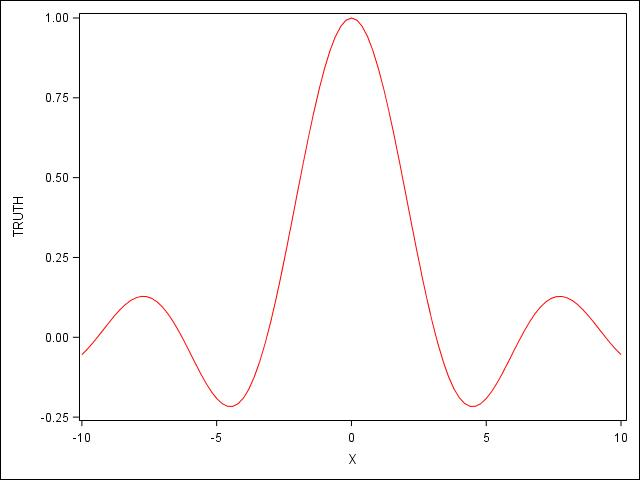
\includegraphics[width=5cm]{groundtruth.jpeg} }}%
    \qquad
    \subfloat[Observed data]{{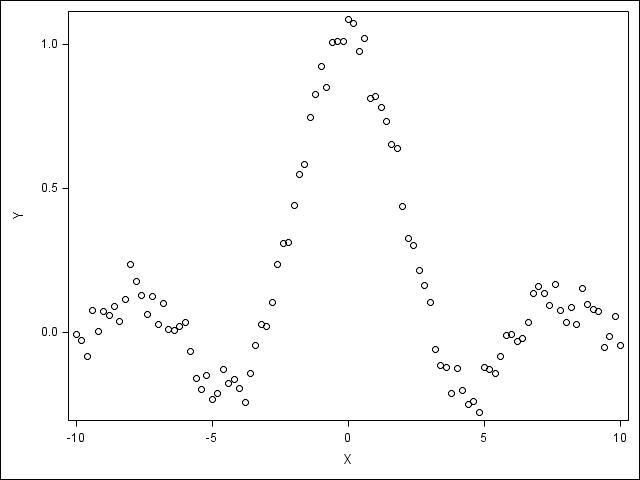
\includegraphics[width=5cm]{observeddata.jpeg} }}%
    \caption{Example variance ground truth compared to observed data}%
    %\label{fig:example}%
\end{figure}
So if $\sigma^2$ is chosen for the above using a Gaussian kernel with a value of $\sigma^2=.05$ compared to $\sigma^2=50$ underfit and overfit are shown
\begin{figure}[H]
    \centering
    \subfloat[$\sigma^2=.05$]{{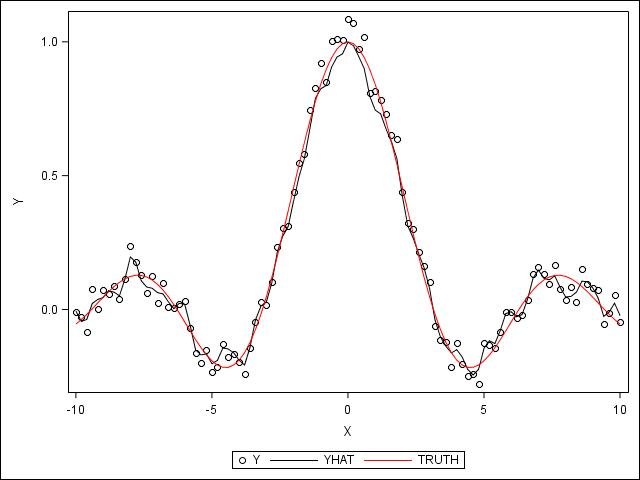
\includegraphics[width=5cm]{sigmap05.jpeg} }}%
    \qquad
    \subfloat[$\sigma^2=50$]{{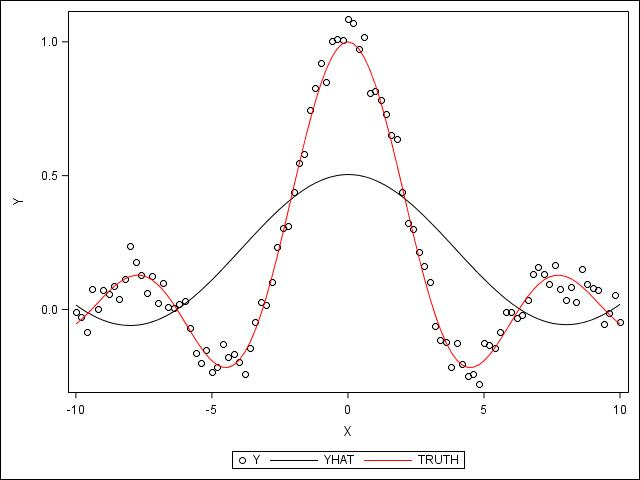
\includegraphics[width=5cm]{sigma50p.jpeg} }}%
    \caption{Overfit and underfit by suboptimal $\sigma$ choices}%
    %\label{fig:example}%
\end{figure}

The bigger issue, of course, is interpretability of the model. 
Even with an accurate classifier (which may be good for a gambler)
how does a coach know what to change on the team to increase the chance.
Here comparing NBA classification models and showing the p-values from a logistic regression
\begin{figure}[H]
    \centering
    \subfloat[Comparison]{{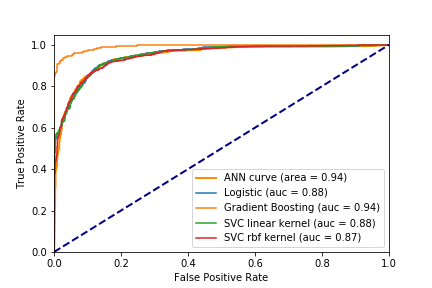
\includegraphics[width=5cm]{overlay.png} }}%
    \qquad
    \subfloat[Pvalues]{{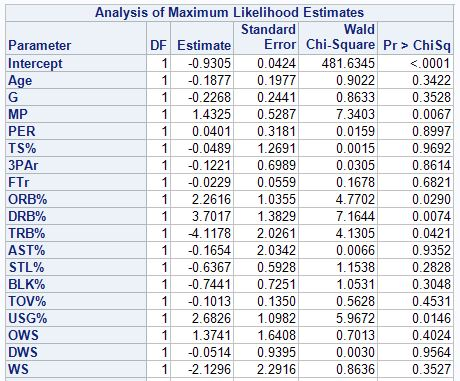
\includegraphics[width=5cm]{logisticpvalues.jpg} }}%
    \caption{Classifier comparison and predictor interpretation}%
    %\label{fig:example}%
\end{figure}

While all the models are good, the Neural Network performed the best. However, the Logistic Regression gives the coach the most information, from the subset above going for blocks may be a great crowd pleaser, but getting defensive rebounds is the way to get to the playoffs!

\subsection{Regression} 
Regression is another type of supervised learning in which the output of the algorithm or hypothesized prediction is a real or continuous value. In terms of predicting NBA outcomes, Support Vector Regression and Linear Regression will be predicting the player's efficiency rating (PER). 

\textbf{\textit{Support Vector Machine}} can be used for classification, but can also be used as a regression method by using the same set of principles with few modifications.
In Support Vector Regression a margin of tolerance, $\epsilon$ - epsilon, is set in approximation to the \textit{SVM}.
The goal is to find a function $f(x)$ that does not deviate from $y_n$ by a value greater than the epsilon for each training point $x$.
While the idea of minimizing error and individualizing the hyperplane remains consistent with \textit{SVM}, one modification is that a part of that error is tolerated.
If a data set is not linearly separable, it is usually mapped into a feature space of higher dimensions using a kernel function.
In this project two such kernel tricks were used with \textit{SVR}. They are as follows:

\begin{center}
Assume ${\bf x}=[x_1,\cdots,x_n]^T$, ${\bf z}=[z_1,\cdots,z_n]^T$

\textbf{Linear Kernel}, $K({\bf x},{\bf z})={\bf x}^T {\bf z}=\sum_{i=1}^n x_1z_1$

\textbf{RBF Kernel}, $K({\bf x},{\bf z})=e^{-||{\bf x}-{\bf z}||^2/2\sigma^2}$
\end{center}
 
\textbf{\textit{Linear Regression}} models the distribution of a continuous response variable \(Y_i\) of subject \(i\) in relation to one or more subject specific explanatory variables. 
Since the distribution of our response variable \textit{Salary}, $Y$, is related to several explanatory variables X\(_{\text{1}}\), X\(_{\text{2}}\), \ldots{}, we used Multiple Linear Regression, which can be expressed by $Y_i=\beta_0+\beta_1\,X_{i1}+\cdots+\beta_p\,X_{ip}+\epsilon_i$

\section{\ Experiment Setup}

\subsection{Dataset}
Our dataset collected from \cite{NBA} comprises of individual player statistics for the years 1978 to 2016. There were 17263 records of 107 features in this dataset. While many of the features like \texttt{3PAr}, \texttt{FTr} were from the original game stats, some features including \texttt{VORP}, \texttt{WS} were derived using expressions based on the original features. In order to avoid multicollinearity among the predictors, we selected the features based on their VIFs. The filtered dataset still contained large set of features. So, to avoid the curse of dimensionality, we performed Principal Component Analysis and reduced the dimension while preserving the variance. The details of the pre-processing is explained in the following subsection.

\subsubsection{Data Pre-processing}

In the first step, records with any of the values missing were removed from the data. Then the features that had details about players identification like \texttt{Player}, \texttt{PlayerId} and features like \texttt{Production}, \texttt{TrueTalent} that are irrelevant to the study were removed. In total 8 such features were dropped from the dataset.

\begin{table}[H]
\caption{Statistics and VIFs of the selected features}
  \label{table:Statistics and VIFs}
  \centering
\begin{tabular}{@{}lrrrrrr@{}}
\toprule
                & \multicolumn{1}{c}{Mean} & \multicolumn{1}{c}{Std Dev.} & \multicolumn{1}{c}{Minimum} & \multicolumn{1}{c}{Median} & \multicolumn{1}{c}{Maximum} & \multicolumn{1}{c}{VIF} \\ \midrule
OWS             & 1.265                    & 2.069                        & -3.100                      & 0.400                      & 15.200                      & 9.007                   \\
G               & 48.900                   & 27.416                       & 1.000                       & 54.000                     & 82.000                      & 8.591                   \\
\ldots & & & & & & \\
Tm\_Adj\_1      & -0.272                   & 0.645                        & -2.600                      & -0.300                     & 1.700                       & 1.426                   \\ 
\bottomrule
\end{tabular}
\end{table}

Moreover, for this project, during the data-preprocessing step, a hyperparameter search will also be performed on the original data, therefore this model can also be used to testify if the hyperparameter grid search indeed give the most "wanting" features.

\subsubsection{Feature Selection}
After the initial filtering of the features the dataset consisted of 99 features. As mentioned above, since some of the remaining features could be expressed in terms of others, Variance Inflation Factor was used to check the linear dependence among them. The VIF is calculated as:

$$
VIF_i = \frac{1}{1-R_i^2} \quad , \quad R^2 = 1 - \frac{\sum_i (y_i-\hat{y}_i)^2}{\sum_i (y_i-\bar{y})^2}
$$

As the formula indicates, the Coefficient of determination value is obtained by regressing the predictor on the remaining predictors. A VIF of 1 means that there is no correlation among that predictor and other predictors and a VIF value greater than 10 indicates serious multicollinearity. So we decided to discard predictors with VIF above the Cutoff value of 10. The statistics of the 23 features reatined and their corresponding VIF values are given in the Table~\ref{table:Statistics and VIFs} above. At the end of preprocessing our dataset contained 16543 records of these 23 features.

\subsubsection{Dimensionality reduction}

As the dimension of the pre-processed dataset was still large, we had to perform principal component analysis to compress the data. Since the first eight components explained maximum variance in the data these eight components were chosen to project the data. Table~\ref{table:Table2} shows the first ten records projected on to those eight principal components.

\begin{table}[H]
\caption{Data projected on to Principal Components}
  \label{table:Table2}
  \centering
\begin{tabular}{@{}crrrrrrrr@{}}
\toprule
   & \multicolumn{1}{c}{PC1} & \multicolumn{1}{c}{PC2} & \multicolumn{1}{c}{PC3} & \multicolumn{1}{c}{PC4} & \multicolumn{1}{c}{PC5} & \multicolumn{1}{c}{PC6} & \multicolumn{1}{c}{PC7} & \multicolumn{1}{c}{PC8} \\ \midrule
0  & 1.746                   & 1.362                   & -2.411                  & -0.094                  & -0.235                  & -1.269                  & 0.958                   & -0.661                  \\
1  & 2.379                   & 3.363                   & -0.264                  & 1.574                   & 0.496                   & 0.910                   & 0.618                   & 0.316                   \\
\ldots &&&&&&&& \\
9  & -0.943                  & -2.146                  & -1.774                  & -0.543                  & 0.843                   & 0.596                   & -0.868                  & 0.430                   \\ 
\bottomrule
\end{tabular}
\end{table}

\subsection{Description of Questions}

\subsubsection{Classification}

There are 3 cases being studied in ANN: 1) taking all 103 features as input for the Artificial Neural Network 2) Taking features after the hyperparameter search as input 3) using remaining features from b) and apply Principal Component Analysis (n=3) and feed the 3 principal vectors as input.
For all cases, the number of the input layer is calculated by using the number of input features (which is 103,30,and 3). Then the number of the output nodes from the input layer to the hidden layer is calculated by taking the sum of the number of input nodes plus the number of output node from the output layer (which is 1 for binary classification) and divide by 2. This is of course only an assumption but it is a very conventional guess for deep learning. 

\subsubsection{Regression}

The aim of this part of our study was to identify the performance measures of an NBA player that act as key factors in deciding how much he gets paid.
Also, given the performance of a player on the court, our model can be applied to check if he is overpaid or underpaid.

\begin{table}[H]
\caption{Grid Search Results}
  \label{GridSearch}
  \centering
\begin{tabular}{@{}ll@{}}
\toprule
Regression                & Hyper-parameters  \\ \midrule
SVR (RBF Kernel)            & C=40, epsilon=1           \\
SVR (Linear Kernel)       & C=10,   epsilon=1           \\
\bottomrule
\end{tabular}
\end{table}

The \textit{SVR} models with these parameters were tested along with the linear regression model.
Also the data was further split into five subsets and the performance of all three models were compared. 
Root mean square error and Adjusted R-squared metrics were used to compare the models. 
The models with least RMSE and an Adjusted R-squared closer to 1 was chosen as the best model to study.

\section{Results}

\subsection{Classification}

\begin{figure}[H]
	\center{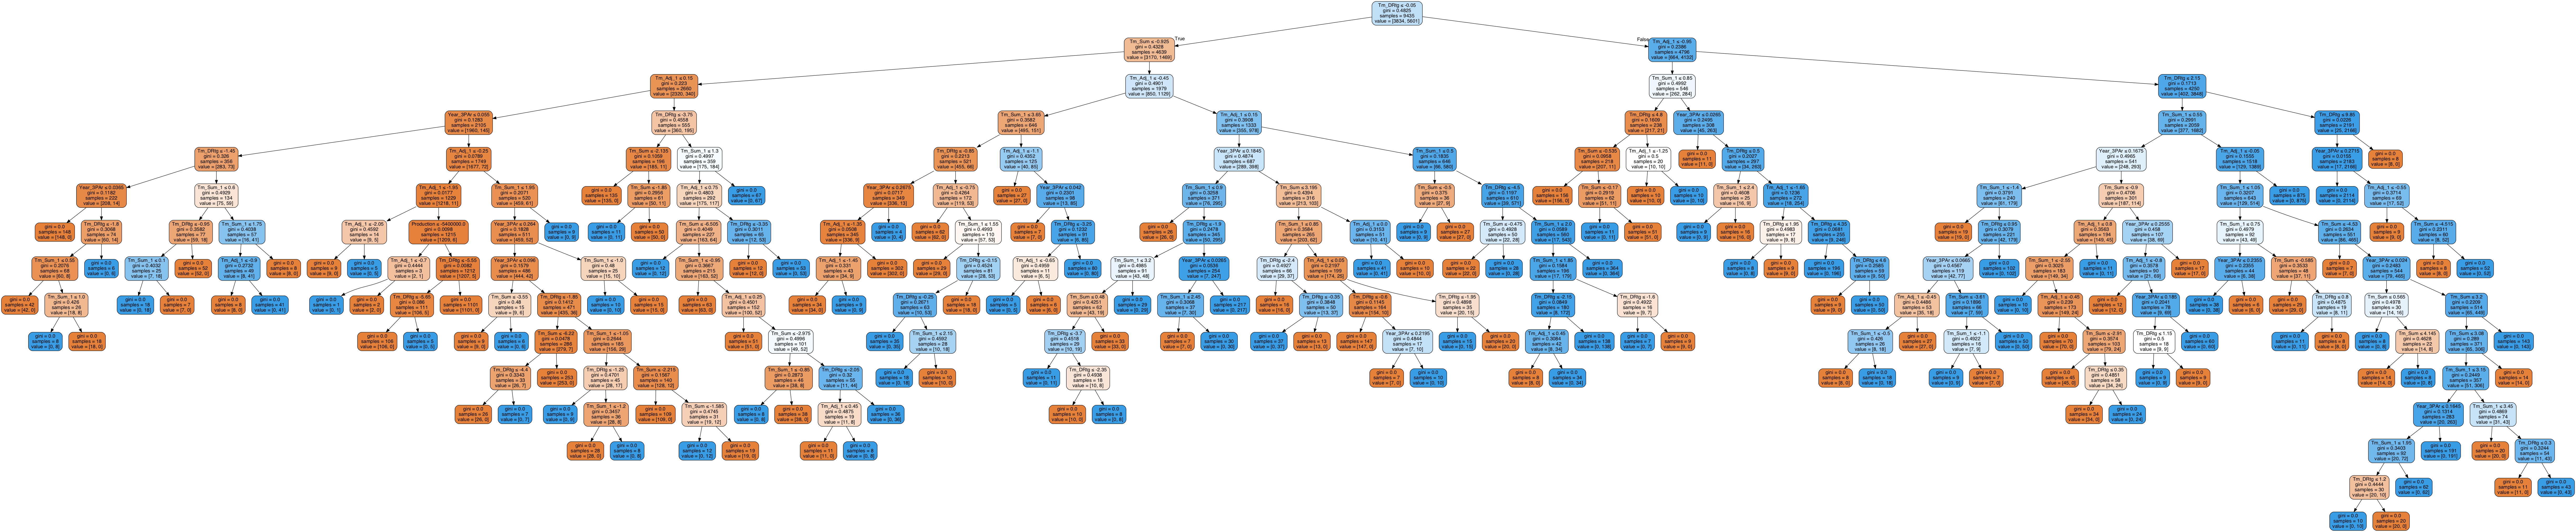
\includegraphics[width=1\textwidth]
		{TreeImage.png}}
	\caption{\label{fig:my-label}Decision Tree Before Pruning}
\end{figure}

\begin{figure}[H]
	\center{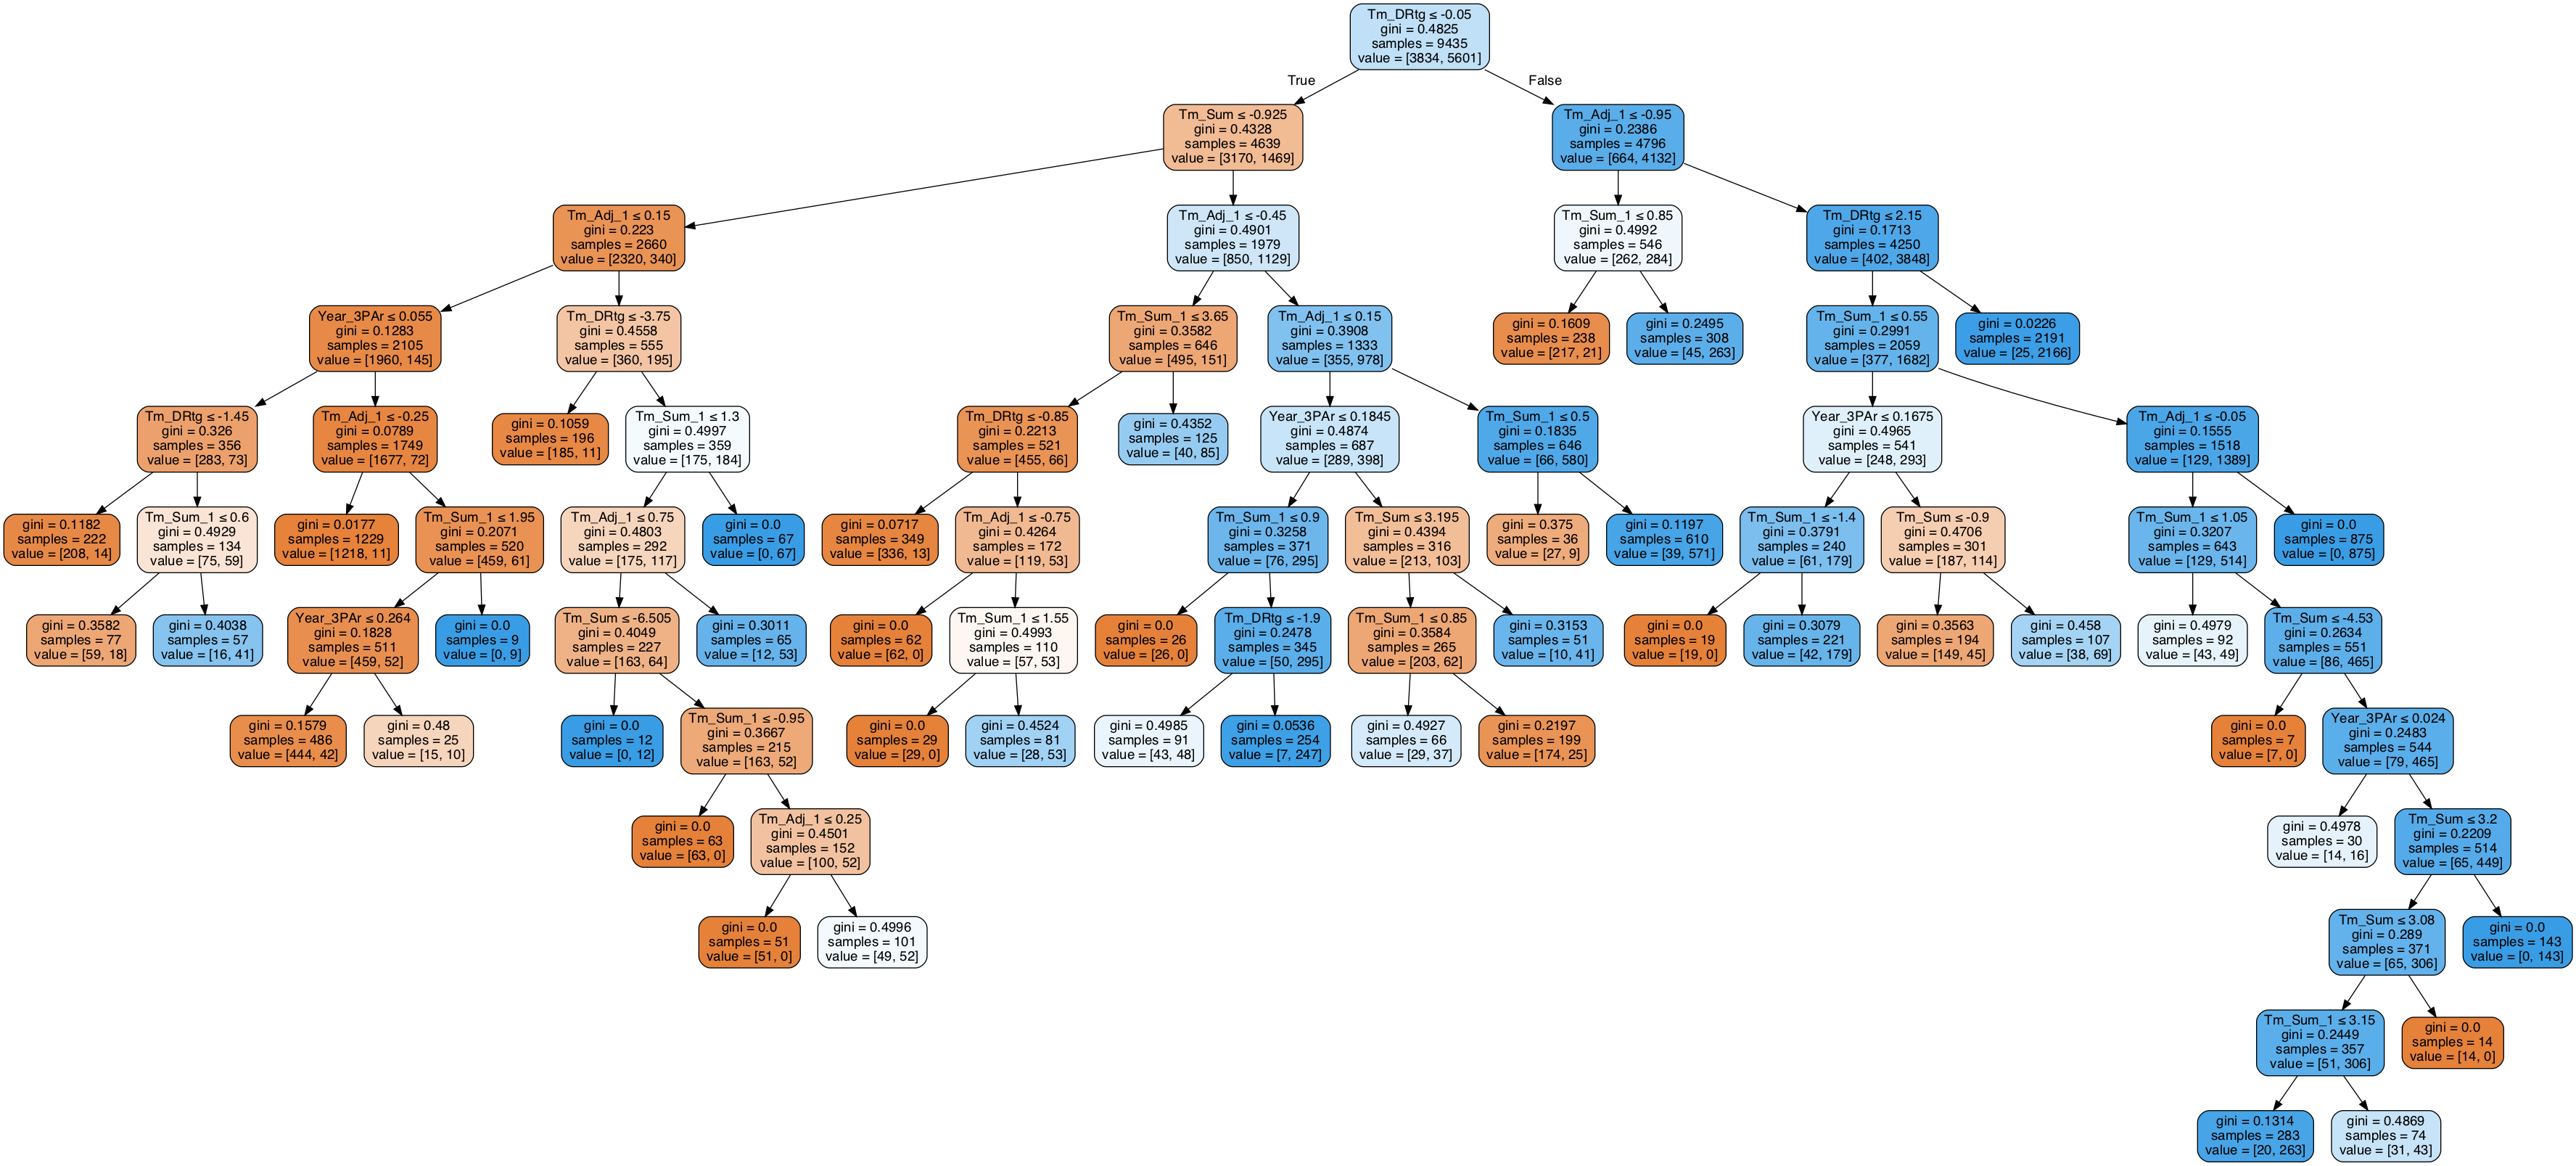
\includegraphics[width=1\textwidth]
		{Prune_TreeImage.png}}
	\caption{\label{fig:my-label}Decision Tree After Pruning, Accuracy = 91\%}
\end{figure}

%  \begin{figure}[H]
%	\center{\includegraphics[width=0.6\textwidth]
%		{ROC.jpg}}
%	\caption{\label{fig:my-label}ROC of different classifiers emphasizing hyperparameters}
%\end{figure}

\begin{table}[H]
\caption{Results after Artificial Neural Network}
  \label{ANN Results}
  \centering
\begin{tabular}{lrrrrrr} % @{}lrrrrrr@{}}
\toprule
  & \multicolumn{3}{c}{After Artificial Neural Network} & \multicolumn{3}{c}{Classification Report (Original Data)} \\ 
  \midrule 
  & Precision & Recall & F1-score & Precision & Recall & F1-score \\ 
\midrule
		0            & 0.83652   & 0.87751 & 0.85652  & 0.83652   & 0.87751 & 0.85652 \\
		1            & 0.92237   & 0.89459 & 0.90827  & 0.92237   & 0.89459 & 0.90827  \\
		Micro Avg    & 0.88809   & 0.88809 & 0.88809   & 0.88809   & 0.88809 & 0.88809 \\
		Macro Avg    & 0.87944   & 0.86605 & 0.88240  & 0.87944   & 0.86605 & 0.88240\\
		Weighted Avg & 0.88969   & 0.88809 & 0.88857  & 0.88969   & 0.88809 & 0.88857 \\
	\end{tabular}
\end{table}

\begin{table}[H]
	\caption{Confusion Matrix, Fail=Missed Playoffs, Success=Made Playoffs}
	\begin{tabular}{lrrrrrr}
	\toprule
	& \multicolumn{2}{c}{Original Data} & \multicolumn{2}{c}{HyperParm Search Data} & \multicolumn{2}{c}{HyperParm Search PCA}\\
\midrule	
		Ground Truth/Prediction & Fail & Success & Fail & Success & Fail & Success \\
		Missed Playoffs                        & 788             & 110             & 764             & 134         & 336             & 532              \\
		Making Playoffs                        & 154             & 1307           & 134             & 1327             & 230             & 1231       
	\end{tabular}
\end{table}

\begin{table}[H]
\caption{Classification Report (Hyperparameter Search Data and HyperParm Search with PCA Data)}
\begin{tabular}{lrrrrrr}
\toprule
& \multicolumn{3}{c}{HyperParm Search} & \multicolumn{3}{c}{HyperParm Search PCA} \\
\midrule
     			& Precision & Recall  & F1-score & Precision & Recall  & F1-score  \\
		0            & 0.85078   & 0.85078 & 0.85078 & 0.61409   & 0.40757 & 0.48996  \\
		1            & 0.90828   & 0.90828 & 0.90828    & 0.698247   & 0.84257 & 0.76365 \\
		Micro Avg    & 0.88639   & 0.88639 & 0.88639   & 0.67698   & 0.67698 & 0.67698   \\
		Macro Avg    & 0.87953   & 0.87953 & 0.87953   & 0.65617   & 0.62507 & 0.62680 \\
		Weighted Avg & 0.88639   & 0.88639 & 0.88639  & 0.66621   & 0.67698 & 0.65946 
\end{tabular}
\end{table}


\subsection{Regression}
After tuning the hyperparameters of the \textit{SVR} models using the grid search, a five-fold cross validation was performed on the dataset to test the models.
The results from these tests are given in the Table~\ref{table:Preliminary results} below. 
As it can be observed in that table the \textit{SVR} with RBF kernel performed better than the linear models. 
The reasons for the under performance of the linear models have been studied and documented below. 

\begin{table}[H]
\caption{5-fold Cross Validation Test Results}
  \label{table:Preliminary results}
  \centering
\begin{tabular}{@{}llll@{}}
\toprule
Model               & RMSE    & R-squared & Adjusted-R-squared \\ \midrule
Linear Regression   & 2.53509 & 0.55308   & 0.55210            \\
SVR (Linear Kernel) & 2.62244  & 0.52238   & 0.52134            \\
SVR (RBF Kernel)    & 2.00159 & 0.72144    & 0.72084            \\ \bottomrule
\end{tabular}
\end{table}

The significance of features in estimating the salaries of the players was also studied and has been expressed using a pie-chart shown in Figure~\ref{fig:reg_chart}. 
According to this chart our model has identified features like \texttt{MPG}, \texttt{Yrs\_Exp}, \texttt{STL} and \texttt{TOPG} as some of the key features that play an important role in deciding a player's remunerations.

\begin{figure}[H]
	\centering
	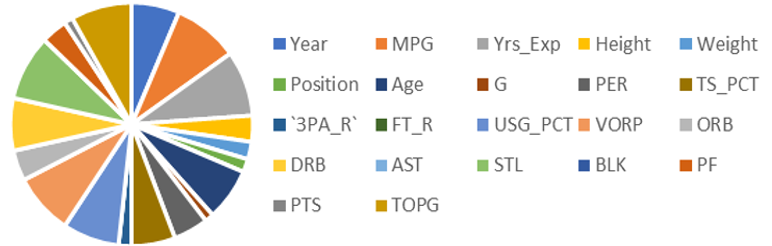
\includegraphics[width=\textwidth] {reg_fig1_pie_chart.PNG}
	\caption{Pie-chart representing the significance of features in predicting the salary of a player}
	\label{fig:reg_chart}
\end{figure}

\subsubsection{Heteroskedasticity}
To investigate the reason why the linear models did not perform well we studied the original Fitted vs Residuals plot that is shown in the left of the Figure ~\ref{fig:reg_plot}.
It can be observed that the residuals are varying systematically (in this case increasing) along the values of the predicted variable.
This condition is called Heteroskedasticity. 
Since this condition violates the Homoskedasticity assumption (ie. same variance across all values of the independent variables), an assumption that is central to linear regression models, we cannot use
linear regression for estimating our target variable.
To overcome this problem we needed to transform our predicted variable \texttt{Salary}.
A logarithmic transformation of this variable was found to be effective in our case.

\begin{figure}[H]
	\centering
        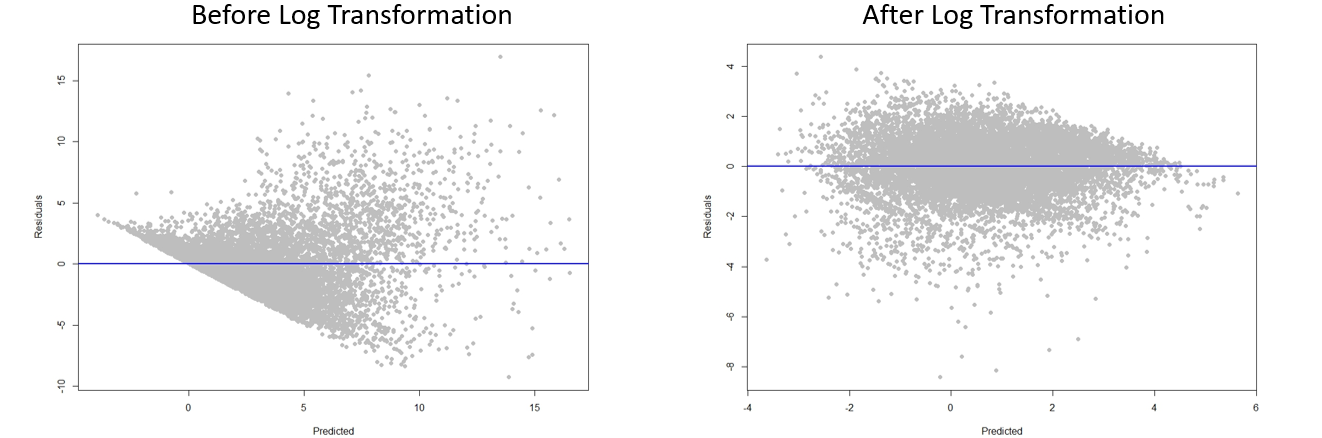
\includegraphics[width=\textwidth] {reg_fig2_fit_res.PNG}
	\caption{Predicted vs Residuals plot before and after Log transformation}
	\label{fig:reg_plot}
\end{figure}

The plot in the right of the Figure~\ref{fig:reg_plot} shows that residuals are distributed well along the predicted values without expressing any increasing or decreasing patterns after the 
log transformation of our response variable. Now the Homoskedasticity assumption is valid and linear regression can be applied to study our target variable.
By applying this transformation and by trying various combinations of predictors we were able to improve the performance of our linear models.

\section{Conclusions}

Clearly machine learning techniques can over-fit training data leading to an art rather than a science of building 
a better predictive model. We hope future research will further refine this fascinating field, in particular, 
using, to the extent possible, more mathematical rigor rather than random re-sampling to draw conclusions (which is why the authors much prefer SVM to ANN, with a stronger foundation in theory and using QP rather than simple back prop refitting randoms, in its rigor and  to ANN.

\begin{enumerate}
	\item Using ANN shows good result for prediction NBA playoffs (0.942)
	\item After hyperparameter search, with only 30 features left, result do not change much and CPU usage for learning progress has a significant decrease
	\item Hyperparameter Optimization in this project is successful 
\end{enumerate}

%\section*{Acknowledgments}

%The authors wish to thank Dr. Min Chi for her guidance and oversight of our research.

\nocite{Povich}
\nocite{Vanhoucke}

\bibliographystyle{abbrv}
\bibliography{NBAPredictionsProject}


\footnotetext{Github Link: \url{https://github.com/csc522nbagroup/playoffsandsalary}}

\end{document}